\documentclass[tikz, border=1cm]{standalone}

\usepackage{tkz-euclide}

\definecolor{facebook}{RGB}{59,89,152}
\definecolor{youtube}{HTML}{90030c}


\begin{document}
	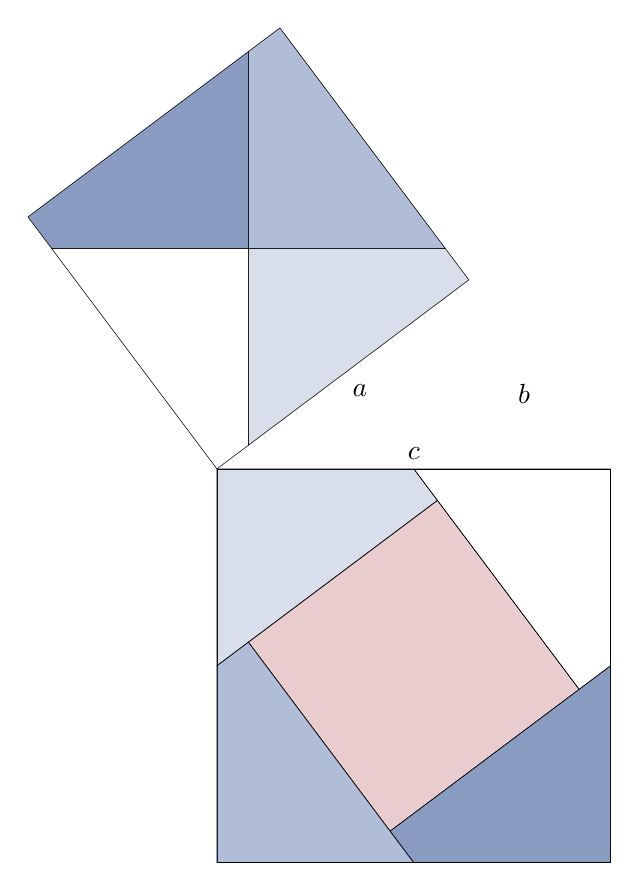
\begin{tikzpicture}[scale=1]
		\tkzDefPoints{0/0/A, 5/0/B}
		\tkzDefSquare(A,B)\tkzGetPoints{C}{D}
		
		\tkzDrawPolygon(A,B,C,D)
		
		\tkzDefMidPoint(A,C)\tkzGetPoint{E}

		
		\tkzDefPointsBy[rotation=center E angle {atan(3/4)}](A,B,C,D){a,b,c,d}

		
		\tkzDefPointsBy[homothety=center E ratio 3/5](a,b,c,d){A',B',C',D'}
		\tkzDrawPolygon[fill=youtube,fill opacity=.2](A',B',C',D')
		
		\tkzInterLL(A',B')(B,C)\tkzGetPoint{F}
		\tkzInterLL(B',C')(C,D)\tkzGetPoint{G}
		
		\tkzDrawPolygon[](B',F,C,G)
		
		\tkzDefPointsBy[translation=from B' to D](F,C,G){H,I,J}
		
		\tkzDrawPolygon[](D,H,I,J)
		
		\foreach \i in {1,2,3}{
			\tkzDefPointsBy[rotation=center E angle 90*\i](B',F,C,G){}
			\tkzDrawPolygon[fill=facebook, fill opacity=.2*\i](B'',F',C',G')
			\tkzDefPointsBy[rotation=center I angle 90*\i](D,H,J){D\i,H\i,J\i}
			\tkzDrawPolygon[fill=facebook, fill opacity=.2*\i](D\i,H\i,I,J\i)
		}
	
		\tkzDrawSquare[fill=youtube,fill opacity=.2](D1,C)
		
		
		\tkzLabelSegment[below right](D,D1){\(a\)}
		\tkzLabelSegment[below left](C,D1){\(b\)}
		\tkzLabelSegment[above](C,D){\(c\)}
	\end{tikzpicture}
\end{document}